% =====================================================================
% COMP 5116 project report -- Control Tower / DriftLedger
% Uses the course template (ProjReportTemplate: stylefile.sty = NeurIPS
% 2023 style, 10pt built in, loads natbib and sets the page layout).
% Compile on Overleaf with report/stylefile.sty and report/references.bib.
% Page budget (12--14 pages total, references <= 2 pages):
%   title+abstract 0.5 | intro 1.25 | related 1.25 | approach 3.5
%   experiments 4.25 | conclusion 0.5 | references 1.5
% =====================================================================
\documentclass{article} % For LaTeX2e
\PassOptionsToPackage{numbers,sort&compress}{natbib}
\usepackage[preprint]{stylefile}
\usepackage{times}
\usepackage{hyperref}
\usepackage{url}

\usepackage[T1]{fontenc}
\usepackage[utf8]{inputenc}
\usepackage{amsmath,amssymb}
\usepackage{graphicx}
\usepackage{booktabs}
\usepackage{xcolor}
\usepackage{tikz}
\usetikzlibrary{positioning,arrows.meta}

\newcommand{\todo}[1]{\textcolor{red}{[TODO: #1]}}

\title{Control Tower: A Drift-Aware, Explainable Continual-Learning System\\
for Fraud and Journal-Entry Risk Monitoring in Banks}
\author{%
  Bonas Djamadjeu Djietcheu\\
  Carleton University\\
  COMP 5116 Machine Learning, Fall 2026
  \And
  Chang Seob Lee\\
  Carleton University\\
  COMP 5116 Machine Learning, Fall 2026
}
\date{}

\begin{document}
\maketitle

% ---------------------------------------------------------------------
\begin{abstract}
\todo{At most 300 words; write in Week 5. Problem, gap (CL for audit
anomaly detection without drift handling, explanations or safe updates),
method (M1--M5), datasets, headline result vs.\ quarterly retraining.}
\end{abstract}

% ---------------------------------------------------------------------
\section{Introduction}\label{sec:intro}
% Budget: 1.25 pages. Owner: Bonaventure (Week 4).
\todo{Problem: fraud losses \citep{acfe2020}, business change breaks fixed
rules and scheduled retraining; Elliptic step-43 shutdown \citep{weber2019elliptic}.}
\todo{Challenges: catastrophic forgetting \citep{kirkpatrick2017overcoming};
regulatory need for auditable, reversible updates \citep{osfi2025e23}.}
\todo{Contributions (bullet list): masked-feature continual detector; drift-vs-anomaly
gate; per-field reason codes with analyst feedback; canary rollback; open benchmark.}

% ---------------------------------------------------------------------
\section{Related Work}\label{sec:related}
% Budget: 1.25 pages (two subsections of about 0.6 page each).
\subsection{Continual learning}\label{sec:related-cl}
% Owner: Bonaventure (Week 2).
Continual learning (CL) studies models that are trained on a sequence of
tasks or data distributions, called experiences, without access to all past
data. The central problem is catastrophic forgetting: when a neural network is
fine-tuned on new data, performance on earlier data drops sharply. Two families
of methods are relevant to our setting. Regularisation methods constrain how
far the parameters may move. Elastic Weight Consolidation (EWC)
\citep{kirkpatrick2017overcoming} adds a quadratic penalty that anchors each
parameter to its value after the previous task, weighted by a diagonal
approximation of the Fisher information, so that parameters that mattered for
old tasks change less. Replay methods instead keep a small memory of past
samples and mix them into training on new data; \citet{rolnick2019experience}
showed that this simple strategy strongly reduces forgetting. Replay works well
in practice, but storing raw records is a concern when the data are financial
transactions, which is why our memory component (M2) treats the buffer size and
the selection rule as design choices. Open-source libraries such as Avalanche
\citep{lomonaco2021avalanche} provide standard benchmarks, strategies and
metrics, which makes CL methods easier to compare under a common protocol.

Most CL research targets supervised classification on image benchmarks.
\citet{pezze2022continual} study how CL strategies carry over to anomaly
detection, where the model learns what normal data look like and the notion of
normal itself changes across experiences; their experiments use image data
rather than tabular records. Closest to our work, \citet{hemati2022continual}
apply CL to unsupervised anomaly detection in continuous auditing. They train a
one-hot-encoded autoencoder on city payment data split into ten experiences, in
which departments gradually disappear under linear, exponential or instant
decay, and they inject global and local anomalies. They compare training on
the single last experience (SEL), joint training on all experiences (JEL), and
the CL strategies sequential fine-tuning (SFT), EWC and experience replay (ER).
JEL gives fewer false positives than SEL, and the CL strategies come close to
JEL without retraining on the full history. We use this setup as our baseline
and reproduce SEL and JEL in Table~\ref{tab:baselines}.
\citet{schreyer2022federated} extend the same line of work to federated CL, in
which several audit clients learn a shared anomaly detector over time without
pooling their accounting data.

These studies show that forgetting is a real problem for audit anomaly
detectors and that standard CL strategies reduce it. They measure success with
reconstruction losses, however, and they treat every change in the data as
something the model should absorb. They do not separate legitimate business
drift from anomalies, explain alerts at the level of individual fields, use
analyst feedback, or protect production from a harmful update. Our system keeps
the CL core (sequential fine-tuning, EWC and replay with random, diversity and
high-error buffer rules) but places it inside a monitoring loop that adds these
missing parts, and it evaluates the loop with operational measures such as
alert volume at equal recall.

\subsection{Anomaly detection and fraud auditing}\label{sec:related-ad}
% Owner: Chang Lee (Week 2).
Labelled fraud is rare in accounting data, so audit analytics relies mostly on
unsupervised anomaly detection. \citet{schreyer2017detection} train deep
autoencoders on large sets of journal entries and flag entries with a high
reconstruction error. They distinguish global anomalies, which carry unusual
attribute values, from local anomalies, which combine common values in an
unusual way, and they one-hot encode categorical attributes. Research on deep
models for tabular data offers richer representations.
\citet{gorishniy2021revisiting} show that a feature tokenizer, which maps each
categorical or numerical feature to its own embedding, combined with a
transformer gives a strong baseline, and that tuned MLP and ResNet models are
competitive with more complex architectures. For anomaly detection,
\citet{thimonier2024beyond} reconstruct masked features of a sample using the
other samples in the training set, and use the reconstruction error as the
anomaly score. Our masked-feature model (Figure~\ref{fig:architecture}) follows
the same masking idea with per-field embeddings, but it is a compact MLP that
can be updated continually, and its per-field errors double as reason codes.
Isolation Forest \citep{liu2008isolation} is a widely used non-neural baseline:
it isolates points with random axis-parallel splits, and points with a short
average path length are scored as anomalous. We compare it with three scoring
functions of our own model: reconstruction error, field-level surprisal and
latent distance.

When labels exist, fraud detection becomes supervised learning, often with
gradient-boosted trees such as XGBoost \citep{chen2016xgboost}. 
\citet{dalpozzolo2018credit} model realistic credit-card fraud detection as a
stream with concept drift. Investigators check only the alerts the system raises, so
most labels arrive late and feedback on alerts is biased towards what the model
already flags. They learn separately from the feedback and from the delayed
labels and then combine the two. Our evaluation protocol, a predict-then-learn
stream with delayed labels, follows this view. Drift itself is studied in
data-stream learning: \citet{gama2014survey} survey concept drift adaptation,
and ADWIN \citep{bifet2007adwin} keeps an adaptive window that shrinks when
two sub-windows have significantly different means. Detectors like these
signal that something changed, but not whether the change is a new normal or a
burst of anomalies.

Public financial-crime benchmarks show why the distinction matters. The
Elliptic dataset \citep{weber2019elliptic} contains about 203{,}000 Bitcoin
transactions over 49 time steps. After a dark market shuts down around step 43,
the models in the original study no longer detect new illicit activity, a clear
case of regime change. Because real labelled bank transactions are rarely
available, \citet{altman2023realistic} release synthetic transaction data with
labelled laundering patterns for anti-money-laundering research. Compared with
this body of work, our design treats drift and anomaly as different events. A
gate decides whether a change should update the model, per-field surprisal
yields reason codes that analysts can confirm or reject, and each update is
checked on a canary set and rolled back if it degrades. The individual
components are known; our contribution is their combination in one
continual-learning system and its evaluation with operational measures.

% ---------------------------------------------------------------------
\section{Approach}\label{sec:approach}
% Budget: 3.5 pages. Owner: Bonaventure (Week 3). Dataset descriptions go in Sec. 4, not here.
\todo{Hypothesis: a drift-gated, explainable CL detector cuts alert volume by
$\geq$20\% vs.\ quarterly retraining at equal recall.}
\todo{Figure 2: pipeline (feed $\rightarrow$ score
$\rightarrow$ reasons $\rightarrow$ analyst $\rightarrow$ drift gate $\rightarrow$ update/rollback).}

\subsection{M1: Masked-feature continual detector}
% Figure 1: architecture of the masked-feature model (M1, MaskedFeatureModel).
% Included from main.tex via % Figure 1: architecture of the masked-feature model (M1, MaskedFeatureModel).
% Included from main.tex via % Figure 1: architecture of the masked-feature model (M1, MaskedFeatureModel).
% Included from main.tex via \input{figures/architecture}.
% Needs \usepackage{tikz} and \usetikzlibrary{positioning,arrows.meta}.
\begin{figure}[t]
\centering
\resizebox{\linewidth}{!}{%
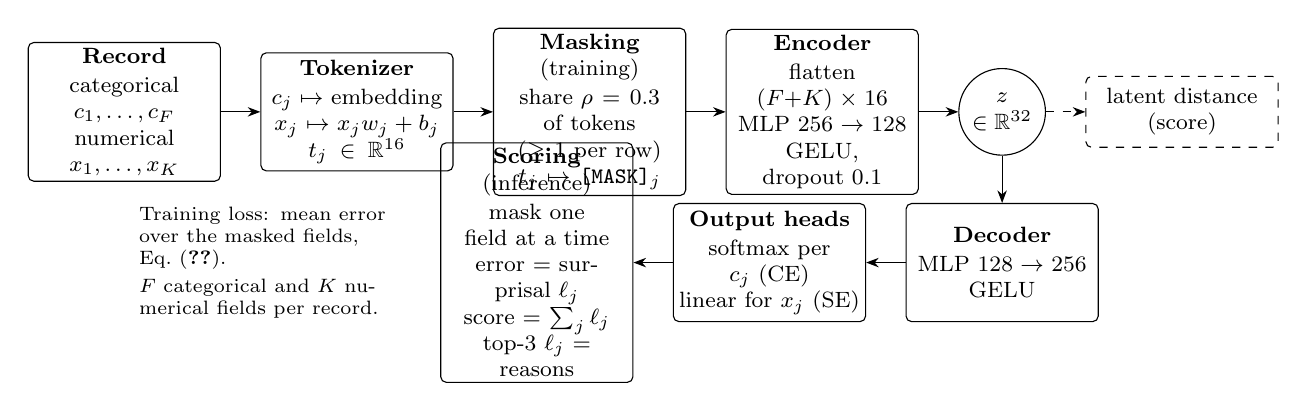
\begin{tikzpicture}[
  font=\footnotesize,
  >={Stealth[length=1.6mm]},
  node distance=6mm and 5mm,
  box/.style={draw, rounded corners=2pt, align=center, text width=2.3cm,
              minimum height=1.5cm, inner sep=2pt},
  latent/.style={draw, circle, align=center, inner sep=1pt, minimum size=1.1cm},
  note/.style={align=left, text width=3.2cm, font=\scriptsize}
]
% ---- row 1: record -> tokens -> masking -> encoder -> latent ----
\node[box] (in) {\textbf{Record}\\[1pt]
  categorical $c_1,\dots,c_F$\\
  numerical $x_1,\dots,x_K$};
\node[box, right=of in] (tok) {\textbf{Tokenizer}\\[1pt]
  $c_j \mapsto$ embedding\\
  $x_j \mapsto x_j w_j + b_j$\\
  $t_j \in \mathbb{R}^{16}$};
\node[box, right=of tok] (mask) {\textbf{Masking} (training)\\[1pt]
  share $\rho = 0.3$ of tokens\\
  ($\geq 1$ per row)\\
  $t_j \mapsto \texttt{[MASK]}_j$};
\node[box, right=of mask] (enc) {\textbf{Encoder}\\[1pt]
  flatten $(F{+}K)\times 16$\\
  MLP $256 \to 128$\\
  GELU, dropout 0.1};
\node[latent, right=of enc] (z) {$z$\\ $\in \mathbb{R}^{32}$};
\node[box, dashed, right=of z, minimum height=0.9cm] (lat) {latent distance\\ (score)};
% ---- row 2 (right to left): decoder -> heads -> scoring ----
\node[box, below=of z] (dec) {\textbf{Decoder}\\[1pt]
  MLP $128 \to 256$\\
  GELU};
\node[box, left=of dec] (heads) {\textbf{Output heads}\\[1pt]
  softmax per $c_j$ (CE)\\
  linear for $x_j$ (SE)};
\node[box, left=of heads] (score) {\textbf{Scoring} (inference)\\[1pt]
  mask one field at a time\\
  error $=$ surprisal $\ell_j$\\
  score $= \sum_j \ell_j$\\
  top-3 $\ell_j$ $=$ reasons};
\node[note, left=of score] (legend) {Training loss: mean error over the
  masked fields, Eq.~\eqref{eq:mfr}.\\[2pt]
  $F$ categorical and $K$ numerical fields per record.};
% ---- arrows ----
\draw[->] (in) -- (tok);
\draw[->] (tok) -- (mask);
\draw[->] (mask) -- (enc);
\draw[->] (enc) -- (z);
\draw[->, dashed] (z) -- (lat);
\draw[->] (z) -- (dec);
\draw[->] (dec) -- (heads);
\draw[->] (heads) -- (score);
\end{tikzpicture}%
}
\caption{Masked-feature model (M1). Each field of a record becomes a
16-dimensional token. During training a share $\rho = 0.3$ of the tokens (at
least one per row) is replaced by a learned per-field \texttt{[MASK]} vector,
and the model reconstructs the masked fields (Eq.~\eqref{eq:mfr}). At
inference each field is masked in turn; its error $\ell_j$ is the per-field
surprisal, the sum over fields is the record's anomaly score and the three
largest $\ell_j$ give the reason codes. The latent $z$ also feeds a
latent-distance score (dashed).}
\label{fig:architecture}
\end{figure}
.
% Needs \usepackage{tikz} and \usetikzlibrary{positioning,arrows.meta}.
\begin{figure}[t]
\centering
\resizebox{\linewidth}{!}{%
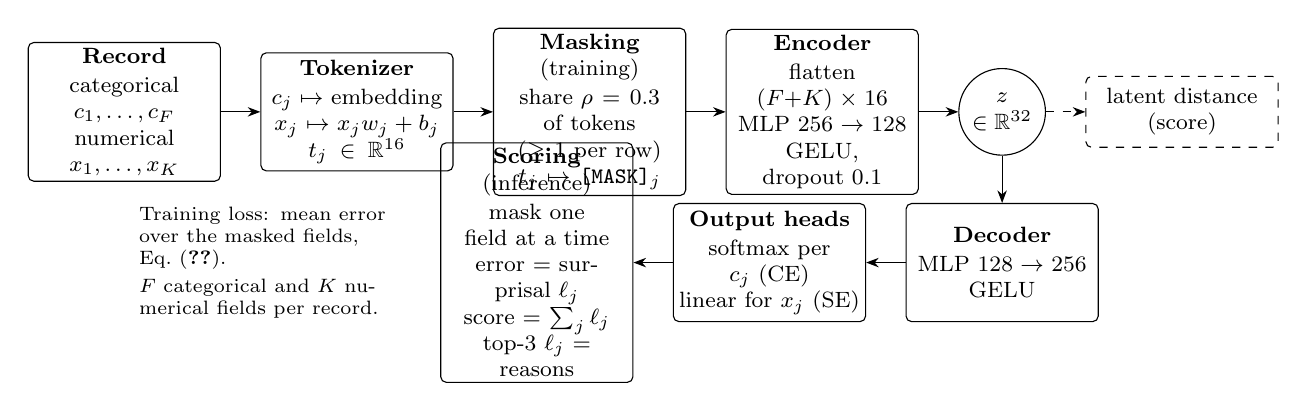
\begin{tikzpicture}[
  font=\footnotesize,
  >={Stealth[length=1.6mm]},
  node distance=6mm and 5mm,
  box/.style={draw, rounded corners=2pt, align=center, text width=2.3cm,
              minimum height=1.5cm, inner sep=2pt},
  latent/.style={draw, circle, align=center, inner sep=1pt, minimum size=1.1cm},
  note/.style={align=left, text width=3.2cm, font=\scriptsize}
]
% ---- row 1: record -> tokens -> masking -> encoder -> latent ----
\node[box] (in) {\textbf{Record}\\[1pt]
  categorical $c_1,\dots,c_F$\\
  numerical $x_1,\dots,x_K$};
\node[box, right=of in] (tok) {\textbf{Tokenizer}\\[1pt]
  $c_j \mapsto$ embedding\\
  $x_j \mapsto x_j w_j + b_j$\\
  $t_j \in \mathbb{R}^{16}$};
\node[box, right=of tok] (mask) {\textbf{Masking} (training)\\[1pt]
  share $\rho = 0.3$ of tokens\\
  ($\geq 1$ per row)\\
  $t_j \mapsto \texttt{[MASK]}_j$};
\node[box, right=of mask] (enc) {\textbf{Encoder}\\[1pt]
  flatten $(F{+}K)\times 16$\\
  MLP $256 \to 128$\\
  GELU, dropout 0.1};
\node[latent, right=of enc] (z) {$z$\\ $\in \mathbb{R}^{32}$};
\node[box, dashed, right=of z, minimum height=0.9cm] (lat) {latent distance\\ (score)};
% ---- row 2 (right to left): decoder -> heads -> scoring ----
\node[box, below=of z] (dec) {\textbf{Decoder}\\[1pt]
  MLP $128 \to 256$\\
  GELU};
\node[box, left=of dec] (heads) {\textbf{Output heads}\\[1pt]
  softmax per $c_j$ (CE)\\
  linear for $x_j$ (SE)};
\node[box, left=of heads] (score) {\textbf{Scoring} (inference)\\[1pt]
  mask one field at a time\\
  error $=$ surprisal $\ell_j$\\
  score $= \sum_j \ell_j$\\
  top-3 $\ell_j$ $=$ reasons};
\node[note, left=of score] (legend) {Training loss: mean error over the
  masked fields, Eq.~\eqref{eq:mfr}.\\[2pt]
  $F$ categorical and $K$ numerical fields per record.};
% ---- arrows ----
\draw[->] (in) -- (tok);
\draw[->] (tok) -- (mask);
\draw[->] (mask) -- (enc);
\draw[->] (enc) -- (z);
\draw[->, dashed] (z) -- (lat);
\draw[->] (z) -- (dec);
\draw[->] (dec) -- (heads);
\draw[->] (heads) -- (score);
\end{tikzpicture}%
}
\caption{Masked-feature model (M1). Each field of a record becomes a
16-dimensional token. During training a share $\rho = 0.3$ of the tokens (at
least one per row) is replaced by a learned per-field \texttt{[MASK]} vector,
and the model reconstructs the masked fields (Eq.~\eqref{eq:mfr}). At
inference each field is masked in turn; its error $\ell_j$ is the per-field
surprisal, the sum over fields is the record's anomaly score and the three
largest $\ell_j$ give the reason codes. The latent $z$ also feeds a
latent-distance score (dashed).}
\label{fig:architecture}
\end{figure}
.
% Needs \usepackage{tikz} and \usetikzlibrary{positioning,arrows.meta}.
\begin{figure}[t]
\centering
\resizebox{\linewidth}{!}{%
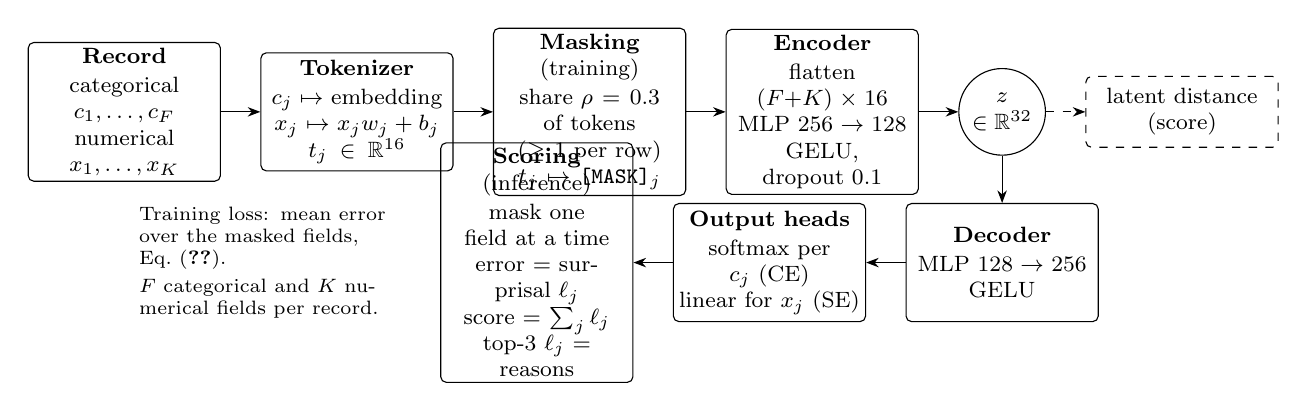
\begin{tikzpicture}[
  font=\footnotesize,
  >={Stealth[length=1.6mm]},
  node distance=6mm and 5mm,
  box/.style={draw, rounded corners=2pt, align=center, text width=2.3cm,
              minimum height=1.5cm, inner sep=2pt},
  latent/.style={draw, circle, align=center, inner sep=1pt, minimum size=1.1cm},
  note/.style={align=left, text width=3.2cm, font=\scriptsize}
]
% ---- row 1: record -> tokens -> masking -> encoder -> latent ----
\node[box] (in) {\textbf{Record}\\[1pt]
  categorical $c_1,\dots,c_F$\\
  numerical $x_1,\dots,x_K$};
\node[box, right=of in] (tok) {\textbf{Tokenizer}\\[1pt]
  $c_j \mapsto$ embedding\\
  $x_j \mapsto x_j w_j + b_j$\\
  $t_j \in \mathbb{R}^{16}$};
\node[box, right=of tok] (mask) {\textbf{Masking} (training)\\[1pt]
  share $\rho = 0.3$ of tokens\\
  ($\geq 1$ per row)\\
  $t_j \mapsto \texttt{[MASK]}_j$};
\node[box, right=of mask] (enc) {\textbf{Encoder}\\[1pt]
  flatten $(F{+}K)\times 16$\\
  MLP $256 \to 128$\\
  GELU, dropout 0.1};
\node[latent, right=of enc] (z) {$z$\\ $\in \mathbb{R}^{32}$};
\node[box, dashed, right=of z, minimum height=0.9cm] (lat) {latent distance\\ (score)};
% ---- row 2 (right to left): decoder -> heads -> scoring ----
\node[box, below=of z] (dec) {\textbf{Decoder}\\[1pt]
  MLP $128 \to 256$\\
  GELU};
\node[box, left=of dec] (heads) {\textbf{Output heads}\\[1pt]
  softmax per $c_j$ (CE)\\
  linear for $x_j$ (SE)};
\node[box, left=of heads] (score) {\textbf{Scoring} (inference)\\[1pt]
  mask one field at a time\\
  error $=$ surprisal $\ell_j$\\
  score $= \sum_j \ell_j$\\
  top-3 $\ell_j$ $=$ reasons};
\node[note, left=of score] (legend) {Training loss: mean error over the
  masked fields, Eq.~\eqref{eq:mfr}.\\[2pt]
  $F$ categorical and $K$ numerical fields per record.};
% ---- arrows ----
\draw[->] (in) -- (tok);
\draw[->] (tok) -- (mask);
\draw[->] (mask) -- (enc);
\draw[->] (enc) -- (z);
\draw[->, dashed] (z) -- (lat);
\draw[->] (z) -- (dec);
\draw[->] (dec) -- (heads);
\draw[->] (heads) -- (score);
\end{tikzpicture}%
}
\caption{Masked-feature model (M1). Each field of a record becomes a
16-dimensional token. During training a share $\rho = 0.3$ of the tokens (at
least one per row) is replaced by a learned per-field \texttt{[MASK]} vector,
and the model reconstructs the masked fields (Eq.~\eqref{eq:mfr}). At
inference each field is masked in turn; its error $\ell_j$ is the per-field
surprisal, the sum over fields is the record's anomaly score and the three
largest $\ell_j$ give the reason codes. The latent $z$ also feeds a
latent-distance score (dashed).}
\label{fig:architecture}
\end{figure}

Figure~\ref{fig:architecture} shows the architecture of the masked-feature model.
Each record has categorical fields $c_1,\dots,c_F$ and numerical fields
$x_1,\dots,x_K$. Field $j$ is mapped to a token $t_j\in\mathbb{R}^d$ (an
embedding for categorical fields, $t_j = x_j w_j + b_j$ for numerical ones).
A random mask $m\in\{0,1\}^{F+K}$ hides each field with probability $\rho$
(at least one field per record). The masked token sequence is $\tilde t$, with
$\tilde t_j = u_j$ if $m_j = 1$ and $\tilde t_j = t_j$ otherwise, where
$u_j\in\mathbb{R}^d$ is a learned \texttt{[MASK]} vector for field $j$. The
encoder maps the flattened $\tilde t$ to a latent code $z\in\mathbb{R}^{32}$, and
the decoder and output heads predict every field from $z$. For a mini-batch $B$
the model minimises the mean error over all masked fields in the batch,
\begin{equation}
\mathcal{L}_{\text{rec}}(B) = \frac{\sum_{n\in B}\sum_{j} m^{(n)}_j\,\ell^{(n)}_j}{\sum_{n\in B}\lVert m^{(n)}\rVert_1},\qquad
\ell_j = \begin{cases}-\log p_\theta(c_j \mid \tilde t) & \text{categorical}\\
(\hat x_j - x_j)^2 & \text{numerical}\end{cases}
\label{eq:mfr}
\end{equation}
where $m^{(n)}$ and $\ell^{(n)}_j$ are the mask and the field errors of record $n$,
and $\hat x_j$ is the prediction from $\tilde t$.

\paragraph{Continual training.}
The detector is trained by sequential fine-tuning (SFT) over the experiences
$E_1,\dots,E_N$: the parameters $\theta$ carry over from one experience to the
next, and each experience is trained for a fixed number of epochs with a newly
created Adam optimiser. With EWC \citep{kirkpatrick2017overcoming}, every
mini-batch loss on experience $E_e$ gets a quadratic penalty,
\begin{equation}
\begin{aligned}
\mathcal{L}(B) &= \mathcal{L}_{\text{rec}}(B) + \frac{\lambda}{2}\sum_i \Omega_i\,(\theta_i - \theta^{*}_i)^2,\\
\Omega_i &= \sum_{e' < e} \Omega^{(e')}_i,\qquad
\Omega^{(e')}_i = \frac{1}{|\mathcal{B}_{e'}|}\sum_{b\in\mathcal{B}_{e'}}
\Bigl(\frac{\partial \mathcal{L}_{\text{rec}}(b)}{\partial \theta_i}\Bigr)^{2}.
\end{aligned}
\label{eq:ewc}
\end{equation}
We write $\Omega$ for the diagonal Fisher information because $F$ already
denotes the number of categorical fields. $\Omega^{(e')}$ is estimated at the
end of experience $e'$ from 2{,}048 sampled records of $E_{e'}$, split into a
set $\mathcal{B}_{e'}$ of mini-batches of 64, with dropout switched off and fresh
random masks. The diagonal Fishers of all past experiences are summed, and
$\theta^{*}$ is the snapshot of the parameters after the latest experience. The
penalty is zero during $E_1$, and $\lambda = 10^{4}$. With replay, every epoch of
experience $E_e$ trains on the current experience together with a memory
$\mathcal{M}$ of earlier records,
\begin{equation}
\mathcal{D}_e = E_e \cup \mathcal{M}_{e-1},\qquad |\mathcal{M}_{e-1}| \le 2{,}000,\qquad \mathcal{M}_0 = \emptyset,
\label{eq:replay}
\end{equation}
which is reshuffled into mini-batches each epoch. The memory is refreshed after
every experience by one of the rules of Section~\ref{sec:m2}. Neither EWC nor
replay uses labels, and the two can be combined.

\paragraph{Scoring.}
A trained model scores a record $r$ with one of four functions, where a higher
score means more anomalous. Let $\ell_j(r; m)$ be the error of field $j$ under
mask $m$, $\mathbf{0}$ the empty mask, and $e_j$ the mask that hides field $j$
alone. Then
\begin{align}
s_{\text{rec}}(r) &= \sum_{j} \ell_j(r; \mathbf{0}), &
s_{\text{surp}}(r) &= \sum_{j} \ell_j(r; e_j), \label{eq:score-model}\\
s_{\text{lat}}(r) &= \frac{1}{k}\sum_{z'\in N_k(r)} \lVert z(r) - z'\rVert_2, &
s_{\text{IF}}(r) &= 2^{-\mathbb{E}[h(\phi(r))]/c(\psi)}. \label{eq:score-ref}
\end{align}
The reconstruction error $s_{\text{rec}}$ measures how well the visible fields
are copied through the bottleneck. The field surprisal $s_{\text{surp}}$ asks
instead whether the other fields predict each field, and its per-field terms
$\ell_j(r; e_j)$ give the top-3 reason codes (Section~\ref{sec:m4}). For the
latent distance, $z(r)$ is the latent code with nothing masked and $N_k(r)$ holds
the $k = 10$ nearest latent codes of a reference set $R$ (records of
$E_1,\dots,E_9$, subsampled to at most 20{,}000). Isolation Forest
\citep{liu2008isolation} does not use our model: $\phi(r)$ replaces each
categorical value by its relative frequency in $R$ and appends the numerical
fields, $h$ is the path length in one tree of a forest of 200 trees fitted on
$R$, and $c(\psi)$ is the usual normalisation for trees grown on subsamples of
size $\psi$.

\subsection{M2: Privacy-aware memory}\label{sec:m2}
The replay memory $\mathcal{M}$ of Eq.~\eqref{eq:replay} holds at most
$|\mathcal{M}| = 2{,}000$ records, about 20\% of one experience. It is refreshed
after every experience without using labels, by one of three rules. The
\emph{random} rule is reservoir sampling over all records seen so far: after
$n$ records have been seen, each of them is in memory with the same probability
$|\mathcal{M}|/n$. The other two rules select from a pool
$P_e = \mathcal{M}_{e-1}\cup C_e$, where $C_e$ is a random sample of at most
5{,}000 records of $E_e$; if the pool is no larger than the memory, it is kept
whole. The \emph{diversity} rule runs greedy $k$-center selection on the latent
codes $z$ of the current model. Starting from one random record, it repeatedly
adds the record farthest from those already chosen,
\begin{equation}
r^{\star} = \arg\max_{r\in P_e}\ \min_{s\in\mathcal{M}_e} \lVert z(r) - z(s)\rVert_2,
\label{eq:kcenter}
\end{equation}
until $|\mathcal{M}_e| = 2{,}000$. The \emph{high-error} rule keeps the records
that the current model finds most surprising,
\begin{equation}
\mathcal{M}_e = \operatorname{top}_{|\mathcal{M}|}\bigl\{\, s_{\text{surp}}(r) : r\in P_e \,\bigr\},
\label{eq:higherror}
\end{equation}
that is, the $|\mathcal{M}|$ records of $P_e$ with the highest field surprisal
(Eq.~\eqref{eq:score-model}).
\todo{Memory footprint of the buffer in MB.}
\subsection{M3: Drift versus anomaly}
\todo{ADWIN on latent statistics, distribution distance, regime-change confirmation;
equation for the drift statistic.}
\subsection{M4: Reason codes and feedback}\label{sec:m4}
\todo{Per-field surprisal $\ell_j$ gives the top-3 reasons; feedback re-ranking.}
\subsection{M5: Governance and safety}
\todo{Canary set, versioning, rollback rule, model-card report \citep{mitchell2019model} aligned with E-23.}

% ---------------------------------------------------------------------
\section{Experiments}\label{sec:experiments}
% Budget: 4.25 pages. Setup drafted Week 4 (Chang Lee); results Week 4 (both).
\subsection{Datasets}
\paragraph{City payments.}
We follow the benchmark construction of \citet{hemati2022continual} and use
two public payment ledgers. The Philadelphia City Payments data for fiscal year
2017 (OpenDataPhilly) have 238{,}894 records, of which 180{,}684 belong to the
ten departments with the most payments. The Chicago Payments data
(data.cityofchicago.org) have 192{,}175 records with a department, of which
134{,}563 belong to the top ten departments. For Philadelphia we use $F = 7$
categorical fields (\texttt{fm}, \texttt{dept}, \texttt{char\_},
\texttt{sub\_obj}, \texttt{vendor\_name}, \texttt{doc\_ref\_no\_prefix},
\texttt{contract\_number}) and $K = 1$ numerical field
(\texttt{transaction\_amount}). For Chicago we use $F = 6$ categorical fields
(department name, vendor name, contract number, the first four characters of
the voucher number, and the year and month of the check date) and $K = 1$
numerical field (the amount). Categorical values are stored as integer codes,
and amounts are min-max scaled to $[0, 1]$. The top ten Philadelphia
departments are, by number of payments, 25, 10, 22, 28, 14, 52, 23, 11, 42
and 12; in Chicago they are Family and Support Services, General Services,
Aviation, Public Health, Transportation, Water Management, Human Resources,
Planning and Development, Fleet and Facility Management, and Buildings.

\paragraph{Experiences and decay.}
Each city is split into $N = 10$ experiences. Every department contributes a
disjoint slice of 1{,}000 records to each experience, of which a share drawn
from $U[0.9, 1]$ is kept. The exception is the target department $A'$, the
second largest in each city (department 10 in Philadelphia, General Services
in Chicago), which is being discontinued: it keeps a scheduled share of its
slice. The share falls from 1 to 0.01 in steps of 0.11 under \emph{linear}
decay; it is roughly multiplied by 0.6 per experience under \emph{exponential}
decay (1, 0.6, 0.36, \dots, 0.01); and it drops to 0 after $E_1$ under
\emph{instant} decay, with 0.01 in $E_{10}$. A \emph{full} scenario without
decay is used for joint training. Departments with fewer than 10{,}000 records
run out of data in $E_7$--$E_{10}$, as in the reference code.
Table~\ref{tab:experiences} gives the resulting stream for the linear scenario.

\paragraph{Injected anomalies.}
As in \citet{hemati2022continual}, we inject two kinds of anomalies. A
\emph{global} anomaly is a copy of a real record whose vendor and one other
categorical field get values that never occur in the data, and whose amount is
set to 2 to 5 times the 99.9th percentile. A \emph{local} anomaly uses only
common values, but each field other than the department is copied from a
record of a different department, which gives combinations that do not occur
in the data. We generate pools of 100 anomalies of each kind, and 10\% of each
pool (10 global and 10 local anomalies) enter the last experience $E_{10}$ only.

\begin{table}[t]
\centering\small
\setlength{\tabcolsep}{4pt}
\caption{Records per experience in the linear-decay scenario
(\texttt{results/experiences\_*\_linear.csv}). $A'$ is the decaying target
department, ``other'' the remaining nine departments, and ``anom.'' the
injected global and local anomalies.}
\label{tab:experiences}
\begin{tabular}{llrrrrrrrrrr}
\toprule
City & Records & $E_1$ & $E_2$ & $E_3$ & $E_4$ & $E_5$ & $E_6$ & $E_7$ & $E_8$ & $E_9$ & $E_{10}$ \\
\midrule
Philadelphia & $A'$  & 1000 & 890 & 780 & 670 & 560 & 450 & 340 & 230 & 120 & 10 \\
             & other & 8500 & 8720 & 8610 & 8450 & 8500 & 8530 & 7269 & 5830 & 5590 & 4429 \\
             & anom. & 0 & 0 & 0 & 0 & 0 & 0 & 0 & 0 & 0 & 20 \\
             & total & 9500 & 9610 & 9390 & 9120 & 9060 & 8980 & 7609 & 6060 & 5710 & 4459 \\
\midrule
Chicago      & $A'$  & 1000 & 890 & 780 & 670 & 560 & 450 & 340 & 230 & 120 & 10 \\
             & other & 8640 & 8460 & 8470 & 8610 & 8560 & 8142 & 5673 & 5012 & 4730 & 4348 \\
             & anom. & 0 & 0 & 0 & 0 & 0 & 0 & 0 & 0 & 0 & 20 \\
             & total & 9640 & 9350 & 9250 & 9280 & 9120 & 8592 & 6013 & 5242 & 4850 & 4378 \\
\bottomrule
\end{tabular}
\end{table}

\paragraph{Deviations from the original setup.}
The authors' encoded files were never published, so we rebuilt the encoding
from the raw data. With the Philadelphia fields above, the one-hot width used
by the baseline autoencoder is 5{,}825, compared with 5{,}588 in the paper. The
Chicago portal now offers only six columns, and the department is filled for
192{,}175 records, whereas the paper used 399{,}158 records with 66 categorical
attributes. Chicago contract numbers take about 31{,}000 values, so we cap them
at 2{,}000 values and merge the rarer ones into a single ``other'' value. We generate the anomalies with the paper's definitions but
without the Faker library used by the authors. For these reasons, Chicago
numbers are not directly comparable with the paper.

\paragraph{Elliptic.}
To test drift on a public financial-crime benchmark, the project will also use
the Elliptic Bitcoin dataset \citep{weber2019elliptic} from Kaggle. It
consists of three tables: transaction features, transaction classes, and the
transaction graph's edge list. It holds 203{,}769 transactions over 49 time
steps, each with anonymised features including its time step, labelled
illicit, licit or unknown. A dark-market shutdown around step 43 provides a
known regime change. A loader that builds a delayed-label stream from these
files has been written and tested on synthetic files; no Elliptic results are
reported yet.
\subsection{Baselines}
\todo{Quarterly retraining, sliding window, SEL, JEL, SFT, EWC, ER, Isolation Forest, XGBoost.}
\subsection{Setup and metrics}
\todo{Predict-then-learn stream with delayed labels; AUPRC, recall at top 1\%,
alert volume at equal recall, recovery time, forgetting, reason-code accuracy,
labels needed, time, memory. Mean $\pm$ std over 5 seeds.}
\subsection{Results}
\todo{Main table generated by script. Table~\ref{tab:baselines} is the Week-1 reproduction (from \texttt{results/summary\_philadelphia\_baseline\_ae.tex}).}
\begin{table}[h]
\centering\small
\caption{Reproduced baselines on Philadelphia, one-hot autoencoder, last experience, mean $\pm$ std over
5 seeds, 100 epochs. Our $\Delta$FP is in our own unit, mean BCE $\times10^{3}$. Paper values are from
\citet{hemati2022continual}, Table~2, which reports $\Delta$FP without stating a unit; our
$\times10^{3}$ values land on the same scale. SEL is identical across decay scenarios because it only sees
the last experience.}
\label{tab:baselines}
\begin{tabular}{llcccccc}
\toprule
Regime & Scenario & $\Delta$FP (ours) & $\Delta$FP (paper) & FP ratio & FN ratio & AUPRC & Recall@1\% \\
\midrule
SEL & linear / exp.\ / inst. & $1.41 \pm 0.04$ & $1.45 / 1.40 / 1.45$ & $0.00 \pm 0.00$ & $0.98 \pm 0.04$ & $0.15 \pm 0.02$ & $0.24 \pm 0.07$ \\
JEL & full & $-1.44 \pm 0.06$ & $-1.36 \pm 0.05$ & $0.05 \pm 0.01$ & $0.62 \pm 0.13$ & $0.36 \pm 0.07$ & $0.69 \pm 0.07$ \\
\bottomrule
\end{tabular}
\end{table}
\subsection{Ablations}
All ablations fine-tune the masked-feature model sequentially over
$E_1,\dots,E_{10}$ for 30 epochs per experience and score $E_{10}$ with the
field surprisal $s_{\text{surp}}$ (Eq.~\eqref{eq:score-model}). The memory holds
$|\mathcal{M}| = 2{,}000$ records and EWC uses $\lambda = 10^{4}$. Values are
mean $\pm$ std over seeds 0, 1 and 2; with three seeds we read differences
smaller than the spread as noise and make no significance claims.

\paragraph{Continual strategy and replay rule.}
Table~\ref{tab:abl-strategies} compares the strategies of Section~\ref{sec:approach}
in the linear scenario, where the injected anomalies appear only in $E_{10}$. On
Chicago, EWC, alone or with random replay, gives the highest AUPRC, roughly
double that of plain fine-tuning, and the most negative $\Delta$FP; this supports
the EWC penalty of Eq.~\eqref{eq:ewc}. On Philadelphia no strategy clearly beats
plain fine-tuning: diversity replay has the highest AUPRC, but within the seed
spread, and EWC, alone or with replay, lowers AUPRC but gives the only negative
$\Delta$FP values.
The best strategy therefore depends on the dataset, which questions a single
default. The memory refreshed after $E_{10}$ (never trained on here) already
shows a risk of the label-free rules: it holds 16.7 (Philadelphia) and 15.3
(Chicago) of the 20 injected anomalies under the diversity rule, and 19.3 and
18.0 under the high-error rule, against 0.3 and 0.0 under random sampling, with
or without EWC.

\begin{table}[t]
\centering\small
\setlength{\tabcolsep}{4pt}
\caption{Strategy ablation, masked-feature model, linear scenario, last
experience $E_{10}$, mean $\pm$ std over 3 seeds, 30 epochs
(\texttt{results/strategies\_\{philadelphia,chicago\}.csv}). $\Delta$FP is in
our own unit, mean BCE $\times10^{3}$. ``EWC + replay'' uses the random rule.}
\label{tab:abl-strategies}
\begin{tabular}{lcccccc}
\toprule
 & \multicolumn{3}{c}{Philadelphia} & \multicolumn{3}{c}{Chicago} \\
\cmidrule(lr){2-4}\cmidrule(lr){5-7}
Strategy & AUPRC & Recall@1\% & $\Delta$FP & AUPRC & Recall@1\% & $\Delta$FP \\
\midrule
None (fine-tuning) & $0.67{\pm}0.09$ & $0.78{\pm}0.10$ & $1.27{\pm}0.44$ & $0.41{\pm}0.05$ & $0.50{\pm}0.00$ & $-3.45{\pm}0.83$ \\
EWC & $0.60{\pm}0.02$ & $0.68{\pm}0.06$ & $-0.68{\pm}0.27$ & $0.80{\pm}0.13$ & $0.88{\pm}0.06$ & $-8.09{\pm}0.94$ \\
Replay, random & $0.67{\pm}0.07$ & $0.80{\pm}0.05$ & $2.82{\pm}0.33$ & $0.59{\pm}0.15$ & $0.67{\pm}0.19$ & $-2.72{\pm}1.36$ \\
Replay, diversity & $0.73{\pm}0.11$ & $0.83{\pm}0.06$ & $1.35{\pm}0.25$ & $0.50{\pm}0.08$ & $0.58{\pm}0.14$ & $-2.83{\pm}0.95$ \\
Replay, high-error & $0.63{\pm}0.06$ & $0.78{\pm}0.03$ & $3.02{\pm}0.48$ & $0.59{\pm}0.18$ & $0.62{\pm}0.23$ & $-3.36{\pm}0.61$ \\
EWC + replay & $0.57{\pm}0.05$ & $0.60{\pm}0.09$ & $-0.38{\pm}0.06$ & $0.81{\pm}0.09$ & $0.92{\pm}0.03$ & $-8.05{\pm}1.15$ \\
\bottomrule
\end{tabular}
\end{table}

\paragraph{Anomaly-aware replay.}
To test whether keeping anomalies out of the memory helps, we add a
\emph{filtered} rule: it drops the top $q = 0.05$ of the candidates by field
surprisal and fills the memory from the rest by reservoir sampling. We run it in
a \emph{linear-spread} scenario, in which 10 global and 10 local anomalies are
injected into each of $E_5,\dots,E_{10}$ (120 in total), so that the memories
used for training can be contaminated; $E_{10}$ is identical to the linear
scenario. Table~\ref{tab:abl-filtered} gives the results. The filter keeps the
replayed memories almost free of injected anomalies, while the diversity and
high-error rules accumulate them, which supports the filter as a contamination
guard. Most of the records it drops, however, are normal. Detection on $E_{10}$
stays within the seed spread of random replay in both cities, so at this
injection rate and with three seeds the lower contamination does not translate
into a measurable gain. We report this as a neutral result.

\begin{table}[t]
\centering\small
\setlength{\tabcolsep}{4pt}
\caption{Replay rules in the linear-spread scenario (20 anomalies injected in
each of $E_5$--$E_{10}$), last experience $E_{10}$, mean $\pm$ std over 3 seeds
(\texttt{results/strategies\_\{philadelphia,chicago\}\_linear\_spread.csv}).
``Inj.\ replayed'' sums the injected anomalies in the memories kept after
$E_1,\dots,E_9$, the ones used for training, so an anomaly kept for several
experiences counts several times. ``Dropped'' is the number of the 120 injected
anomalies removed by the filter.}
\label{tab:abl-filtered}
\begin{tabular}{llcccc}
\toprule
City & Rule & AUPRC & Recall@1\% & Inj.\ replayed & Dropped \\
\midrule
Philadelphia & none (fine-tuning) & $0.655{\pm}0.069$ & $0.75{\pm}0.10$ & -- & -- \\
             & random     & $0.592{\pm}0.045$ & $0.72{\pm}0.08$ & $11.7{\pm}4.7$ & -- \\
             & diversity  & $0.581{\pm}0.058$ & $0.65{\pm}0.05$ & $157.3{\pm}21.0$ & -- \\
             & high-error & $0.574{\pm}0.046$ & $0.63{\pm}0.10$ & $171.7{\pm}28.2$ & -- \\
             & filtered   & $0.584{\pm}0.065$ & $0.68{\pm}0.03$ & $0.0{\pm}0.0$ & $108.0{\pm}3.5$ \\
\midrule
Chicago      & none (fine-tuning) & $0.330{\pm}0.072$ & $0.47{\pm}0.12$ & -- & -- \\
             & random     & $0.491{\pm}0.155$ & $0.58{\pm}0.18$ & $6.7{\pm}7.2$ & -- \\
             & diversity  & $0.487{\pm}0.116$ & $0.55{\pm}0.05$ & $148.7{\pm}40.4$ & -- \\
             & high-error & $0.301{\pm}0.110$ & $0.45{\pm}0.05$ & $117.3{\pm}15.0$ & -- \\
             & filtered   & $0.433{\pm}0.102$ & $0.52{\pm}0.10$ & $3.0{\pm}4.4$ & $84.0{\pm}8.5$ \\
\bottomrule
\end{tabular}
\end{table}

\todo{Remaining ablations: 1 drift gate, 2 scoring function, 4 EWC strength,
5 analyst feedback, 6 mask ratio, 7 percentile calibration, 8 canary rollback.}

% ---------------------------------------------------------------------
\section{Conclusion}\label{sec:conclusion}
% Budget: 0.5 page. Week 5.
\todo{Findings, limits (no real bank labels), path to a shadow-mode pilot.}

% ---------------------------------------------------------------------
\bibliographystyle{abbrvnat}
\bibliography{references}

\end{document}
